\documentclass[a4paper,11pt]{article}
\usepackage{latexsym}
\usepackage{hyperref}
\usepackage{graphicx}
\usepackage[MeX]{polski}
\usepackage[utf8]{inputenc}
\usepackage{geometry}
\usepackage{hyperref}
\usepackage{subcaption}
\usepackage{natbib}
\usepackage[nottoc,numbib]{tocbibind}
 \geometry{
 a4paper,
 left=20mm,
 top=30mm,
 }
\author{Adam Gonstal, Kamil Kolasa, Rafał Kornel, Konrad Maliszewski, Anna Olechowska}
\title{Poszukiwanie mikrosoczewek grawitacyjnych}
\frenchspacing
\newcommand{\ak}{\hspace{0.7 cm}}
\renewcommand{\abstractname}{Abstrakt}
\bibliographystyle{plainnat}
\setcitestyle{authoryear,open={(},close={)}}
\begin{document}
\maketitle
\newpage
\tableofcontents
\newpage
\begin{abstract}
\nocite{*}
\ak Poniżej opisany projekt studencki polegał na analizie fragmentu danych z projektu OGLE III w celu znalezienia zjawisk mikrosoczewkowania grawitacyjnego.  Autorom zostały udostępnione dane z teleskopu w Las Campanas w Chile, dotyczące m.in. pomiarów jasności dla ok. $260$ tysięcy  gwiazd, zbieranych na przestrzeni ok. $6$ lat. W ramach projektu utworzony został algorytm analizujący dane dla każdej gwiazdy i zwracający wykresy zależności jasności od czasu dla tych gwiazd, które według algorytmu mogły dawać efekt soczewki. Około $x\%$ zwróconych gwiazd okazało się rzeczywistymi przypadkami mikrosoczewkowania grawitacyjnego. Ponadto, $y$ ze znalezionych przez algorytm soczewek nie zostały zidentyfikowane przez zespół projektu OGLE III.
\end{abstract}
\section{Wstęp}
\subsection{Wstęp teoretyczny}
\ak Zjawisko soczewkowania grawitacyjnego wynika z zakrzywienia czasoprzestrzeni przez masy znajdujące się w niej. Konsekwencją tego jest poruszanie się promieni świetlnych po zakrzywionych torach, tj. najkrótszych możliwych, w przestrzeni Mińkowskiego. W związku z tym, w sytuacji gdy w okolicach linii łączącej źródło światła (np. galaktykę) z obserwatorem znajdzie się odpowiednio duża masa, światło biegnie omijając taką masę, co przedstawia Rysunek \ref{Fig_1}. 

\begin{figure}[h]
\centering
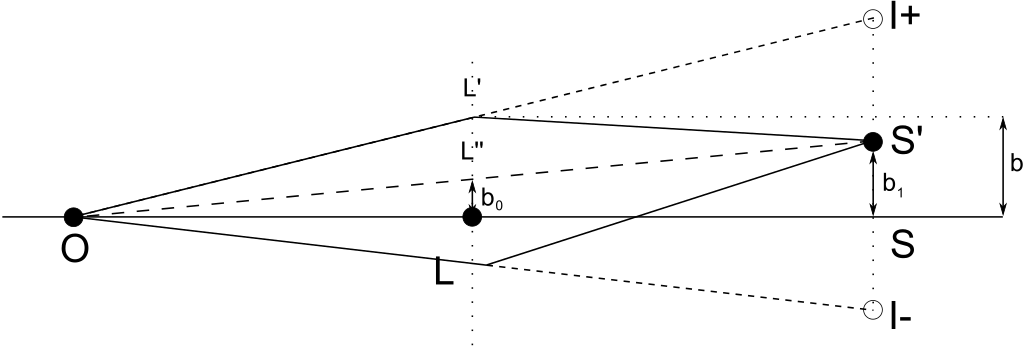
\includegraphics[width=0.9\textwidth]{Fig/Lens.jpeg}
\label{Fig_1}
\caption{Przykład zjawiska soczewkowania, gdzie źródło S' jest obserwowane jako dwa obrazy I+ i I- \citet{Lens}.}
\end{figure}

\ak Obraz źródła widziany przez obserwatora może ulec różnym deformacjom, tj. rozciągnięciu, przemieszczeniu, kilkukrotnemu odbiciu, a także wzmocnieniu, co w przypadku tego projektu jest najistotniejszym aspektem soczewkowania. Przykłady takiego zjawiska przedstawiają Rysunki \ref{Fig_2} i \ref{Fig_3}.
\newpage%UWAGA NEWPAGE
\begin{figure}[h]
\begin{subfigure}{0.5\textwidth}
\centering
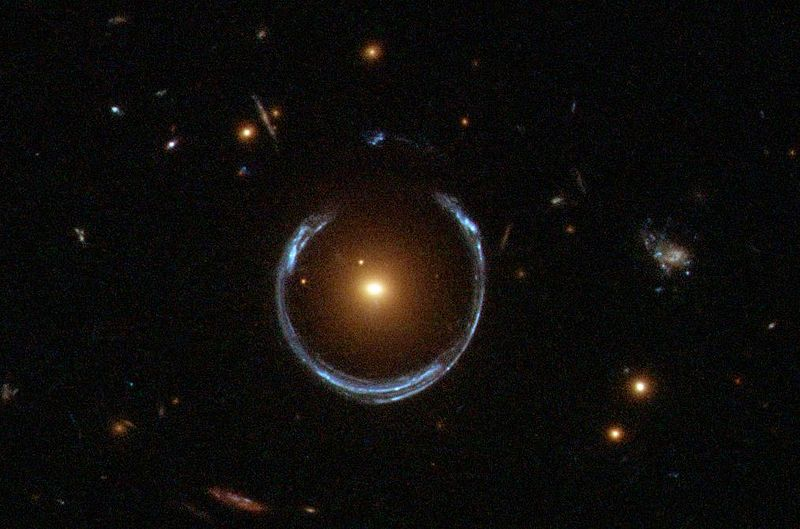
\includegraphics[width=0.9\linewidth,height=5cm]{Fig/Horseshoe.jpeg}
\caption{Galaktyka LRG 3-757 soczewkująca obraz galaktyki znajdującej się za nią \citet{Horseshoe}}
\label{Fig_2}
\end{subfigure}
\hspace{0.5cm}
\begin{subfigure}{0.5\textwidth}
\centering
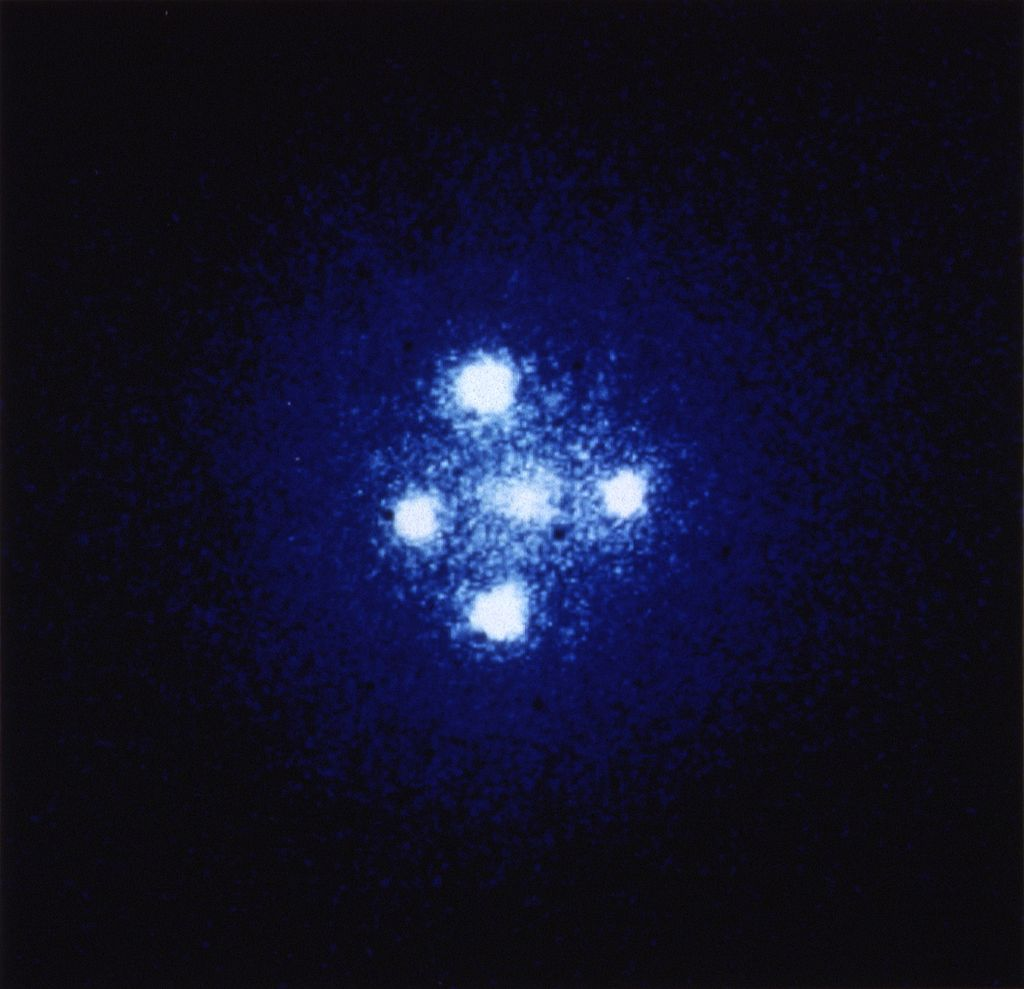
\includegraphics[width=0.9\linewidth,height=5cm]{Fig/Cross.jpeg}
\caption{Kwazar Q2237+030 soczewkowany przez galaktykę ZW 2237+030, tzw. krzyż Einsteina \citet{Cross}}
\label{Fig_3}
\end{subfigure}
\caption{Przykłady deformacji obrazu spowodowane soczewkowaniem grawitacyjnym}
\end{figure}
\ak W szczególnych przypadkach, gdy masa soczewkująca jest stosunkowo nieduża, a jej tor ruchu przecina bądź jest bardzo bliski torowi promieni świetlnych od źródła do obserwatora, efekty deformacji obrazu mają zbyt małe rozmiary kątowe, by udało się je zaobserwować z Ziemi. W takich sytuacjach jedyną obserwowalną konsekwencją zajścia soczewki jest wzmocnienie jasności. Ten specyficzny rodzaj soczewkowania nazywany jest mikrosoczewkowaniem grawitacyjnym. Przykładem jego może być obiekt z pobliskiej galaktyki wysyłający ku Ziemi promieniowanie elektromagnetyczne, na którego drodze znajduje się masywna planeta. Wzmocnienie można wyrazić jako wielkość $\mu$, będącą ilorazem strumienia światła bez wzmocnienia oraz z wzmocnieniem. Ponieważ natężenie światła $I$ jest stałe w czasie, będzie to wyłącznie iloraz kątów bryłowych, z których światło dociera do  obserwatora.\\
\begin{equation}
\centering
\mu=\frac{Id\Omega}{Id\Omega_{0}}=\frac{d\Omega}{d\Omega_{0}}
\label{Eq_1}
\end{equation}
\flushleft
\ak Wzmocnienie można również dobrze opisać za pomocą odległości $u$ źródła światła od soczewki, którą można opisać za pomocą kilku parametrów, które dla danej soczewki można przyjąć jako stałe w trakcie trwania zjawiska. Wspomniane parametry geometryczne mają wpływ na $t_{E}$, tj. czas Einsteina. Wielkość $b$ jest wielkością analogiczną do parametru zderzenia i także jest stała. Czas $t_{0}$ jest momentem największego wzmocnienia, z kolei jedyną zmienną we wzorze \ref{Eq_2} jest czas {t}.
\begin{equation}
\centering
u(t)=\sqrt{\left(\frac{t-t_{0}}{t_{E}}\right)^{2}+b^{2}}
\label{Eq_2}
\end{equation}
\ak Znając już zależność $u(t)$ można powiązać ją ze wspomnianym wcześniej wzmocnieniem $\mu$, tj. wyprowadzić wzór \ref{Eq_3}, zwany także krzywą Paczyńskiego. Przykładową krzywą Paczyńskiego przedstawia Rysunek \ref{Fig_997}. %tutaj ref do krzywej w subsection "Projekt OGLE"
W skali sześciu lat mikrosoczewka trwająca ok. $70$ dni widocznie wyróżnia się skokiem jasności w trakcie trwania zjawiska, co było punktem wyjściowym przy konstrukcji algorytmu i zostanie opisane dokładniej w kolejnych rozdziałach.
\begin{equation}
\centering
\mu(u)=\frac{u^{2}+2}{u\sqrt{u^{2}+4}}
\label{Eq_3}
\end{equation}
\flushleft
\subsection{Projekt OGLE}

\ak Projekt OGLE  tj. ,,Optical Gravitational Lensing Experiment'' jest projektem naukowym prowadzonym w obserwatorium Las Campanas w Chile, przez Obserwatorium Astronomiczne Uniwersytetu Warszawskiego, w ramach którego m.in. wykonywane są pomiary jasności gwiazd, mające na celu poszukiwanie zjawisk mikrosoczewkowania. 

\ak Projekt kierowany jest przez prof. Andrzeja Udalskiego, a jego zasadniczym obszarem obserwacji są rejony w pobliżu centrum naszej galaktyki. Od początku istnienia projektu (kwiecień 1992 roku) zaobserwowano: 20 nowych planet pozasłonecznych, ponad 4000 zjawisk mikrosoczewkowania oraz kilkaset tysięcy nowych gwiazd zmiennych\footnote{Dane ze strony internetowej projektu: \textit{http://www.astrouw.edu.pl/index.php/ogle-artykul}}. Projekt jest aktualnie (od marca 2010 roku) w czwartej fazie realizacji. Poprzednie fazy miały miejsce w latach: 1992-1995 (OGLE-I), 1997-2001 (OGLE-II), 2001-2009 (OGLE-III) i wiązały się ze stosowaniem innych detektorów.
 \\
\textbf{Następny akapit może wrzucić do analizy danych?} 
 \\
\ak Dane na których oparty jest nasz projekt studencki pochodzą z projektu OGLE-III i zawierają \textbf{X} plików tekstowych w, którym jest średnio \textbf{Y} pomiarów jasności w przeciągu 6 lat. Warto wspomnieć tutaj że jakość część pomiarów jest daleka do ideału i musieliśmy posegregować dane czy się nadają do analizy, np. w części plików były pojawiały się tylko jasności gwiazd 99,9 magnitudo co oczywiście nie sama sensu.
\section{Analiza danych}
\subsection{Ogólnie o programie}
\ak Do analizy danych napiliśmy program w języku Python. Dokładny kod znajduje się na naszym git hubie \textbf{[tu link]}. Składa się on z kilku części:
\begin{enumerate}
\item ,,Main'', czyli... 
\item ...
\end{enumerate} 
\subsection{Opis algorytmu}
\ak \textbf{...} Po wyfiltrowaniu wstępnie wszystkich potencjalnie nie nadającej się do obróbki danych tzw. ,,syfów'', program operując już na nowych nie odrzuconych danych oblicza ich parametry, takie jak \textbf{odchylenie standardowe od średniej dla pomiarów jasności tj.  $\sigma_{mag}$} i średnia pomiarów jasności tj. $m_0$. Następnie  sprawdzamy, które pomiary jasności, oznaczenie $m$, spełniają nierówność (tj. są jaśniejsze)
\begin{equation}
m<\sigma_{mag}\cdot A+m_0
\end{equation}  i zliczamy je. Przy czym $A$ jest arbitralnie ustaloną liczbą dodatnią wybraną przez programistę. Następnie z tych punktów spełniających nierówność, liczymy odchylenie standardowe po czasie oznaczenie $\sigma_t$, oraz średni czas $t$ tych punktów.
\\
\ak Jeżeli, teraz nasz plik z danymi zawiera \textbf{{n}} spełniających nierówność (4) i jeżeli $\sigma_t$ jest mniejsze niż \textbf{T}, to program zwraca nam informacje o podejrzeniu że w tym pliku może być soczewka, wraz z wykresem pomiarów jasności, naniesionym czasem $t$. Czas ten informuje nas kiedy, według programu zachodzi soczewka.
\\
\ak Zasadniczą ideą, którą się posługujemy jest fakt, że nasze soczewki będą jaśniejsze niż ,,większość'' pomiarów, przy czym dokładna znaczenie słowa ,,większość'' jest ustalone, przez wybór wartości $A$, np. zakładając że pomiary jasności podlegają rozkładowi Gaussa, co w ogólności nie musi być prawdą np. dla gwiazd mocno zmiennych, dla wartości $A=1$ przewidujemy, że odrzucimy około $67\%+16,5\%=83,5\%$ punktów. 
\\ 
\ak Drugim faktem, który dla nas jest kluczowy jest to informacja, że mikro soczewki nie trwają dłużej niż 100-200 dni.

\section{Rezultaty}
\bibliography{bibliografia}
\end{document}
